\documentclass[12pt]{article}
	\usepackage[margin=1in]{geometry}
	\usepackage[hidelinks, linktoc=all, pagebackref, russian]{hyperref}
	\usepackage{indentfirst}
    \usepackage[russian]{babel}
    \usepackage{subcaption}
   	\usepackage[superscript,biblabel]{cite}
    \usepackage[font=small,labelfont=bf]{caption}
    \usepackage{abstract}
    \usepackage{mathtools}
    \usepackage{cleveref}
    \setlength{\parskip}{0.1cm}   
	\setlength{\parindent}{0.7cm}
    \usepackage{graphicx} % Used to insert images
    \usepackage{adjustbox} % Used to constrain images to a maximum size 
   	\usepackage{color} % Allow colors to be defined
    \usepackage{enumerate} % Needed for markdown enumerations to work
    \usepackage{geometry} % Used to adjust the document margins
    \usepackage{amsmath} % Equations
    \usepackage{amssymb} % Equations
    \usepackage[mathletters]{ucs} % Extended unicode (utf-8) support
    \usepackage[utf8x]{inputenc} % Allow utf-8 characters in the tex document
    \usepackage{fancyvrb} % verbatim replacement that allows latex
    \usepackage{grffile} % extends the file name processing of package graphics 
                         % to support a larger range 
    % The hyperref package gives us a pdf with properly built
    % internal navigation ('pdf bookmarks' for the table of contents,
    % internal cross-reference links, web links for URLs, etc.)
    \usepackage{longtable} % longtable support required by pandoc >1.10


 	
\addto\extrasrussian{%
  \renewcommand{\figureautorefname}{Рис.}%
}
\DeclarePairedDelimiter\bra{\langle}{\rvert}
\DeclarePairedDelimiter\ket{\lvert}{\rangle}
\DeclarePairedDelimiterX\braket[2]{\langle}{\rangle}{#1 \delimsize\vert #2}
\newcommand{\rbrkt}[1]{\left( #1 \right)}
\renewcommand*{\backreftwosep}{ и~}
\renewcommand*{\backreflastsep}{ и~}
\renewcommand*{\backref}[1]{}
\renewcommand*{\backrefalt}[4]{%
\ifcase #1 %
\relax%
\or
(cслыка на стр. [#2])%
\else
(cслыки на стр. [#2])%
\fi
}

\numberwithin{equation}{section}
\setcounter{tocdepth}{3}


	\author{Федоров Глеб, 125}
 	\title{Диплом}

\begin{document}
\maketitle
\tableofcontents
\newpage
\part*{Введение}
\addcontentsline{toc}{part}{Введение}
Квантовый компьютер -- это устройство, хранящее и обрабатывающее информацию в группе квантовых систем, причем обработка информации происходит в результате когерентных взаимодействий систем внутри группы \cite{Lloyd1993}. Каждая квантовая система, как правило, является двухуровневой и носит название ``квантовый бит'' или ``кубит'' (англ. ``qubit'' -- quantum bit). Для осуществления квантового расчета необходимо уметь реализовывать связь между кубитами, управлять состоянием кубитов, сохраняя его чистоту, определять состояние каждого из кубитов в группе и, наконец, изолировать кубиты от окружающей среды, следовательно, в качестве кубитов могут быть использованы любые достаточно изолированные двухуровневые системы, поддающиеся контролю и способные взаимодействовать друг с другом \cite{DiVincenzo1995, DiVincenzo2000, Spiller1996}. В качестве примера можно привести фотоны \cite{Milburn2009}, ионы в ионных ловушках \cite{Cirac1995}, ядерные спины \cite{Kane1998}, атомы в электромагнитных резонаторах\cite{Rempe2008},  электрические системы\cite{Devoret2005} и т.п.

Последние являются одними их самых заманчивых кандидатов на эту роль, если только окажутся подчинены квантовой механике\cite{Devoret1995}. К счастью, явление сверхпроводимости и эффект Джозефсона позволяют наблюдать квантовые эффекты в контурах даже мезоскопического масштаба и создавать так называемые сверхпроводящие (джозефсоновские) кубиты\cite{Clarke2008}. В данной работе проводится исследование одного из них -- потокового сверхпроводящего кубита (впервые предложен в статье\cite{Orlando1999} и назван Flux-кубитом).

Джозефсоновские кубиты имеют два значительных недостатка и одно значительное преимущество в сравнении с микроскопическими кубитами. Первый недостаток касается шума и нарушения чистоты состояния - в силу больших размеров, джозефсоновские кубиты сильнее связываются со средой, что требует дополнительных изысканий в области их изоляции; второй недостаток заключается в том, что в то время как микроскопические кубиты, например, атомы, идентичны друг другу, сверхпроводящие кубиты могут иметь отличия из-за неточностей производства. Для борьбы с этим требуется либо создавать заведомо нечувствительные к дефектам схемы, либо проводить калибровку, в процессе которой параметры цепей измеряются и компенсируются.

Преимущество джозефсоновских кубитов в их гибкости: они могут быть произвольным образом расположены относительно друг друга, а их параметры легко и непрерывно изменяемы в широких пределах. Эта гибкость вместе с некоторыми фундаментальными эффектами\cite{Koch2007} может быть использована для борьбы с первым недостатком, а также предоставляет много вариантов для подстройки параметров, что в значительной степени нивелирует второй недостаток. Далее, накопленный опыт человечества в области изготовления интегральных схем позволит упростить переход к производству реальных устройств, что является очевидным преимуществом в сравнении с другими типами кубитов. Таким образом, скорее всего именно джозефсоновские кубиты и будут применены в первом квантовом компьютере, и именно их следует изучать.

Важно отметить, что сверхпроводящие кубиты могут применяться не только для непосредственного использования в квантовом компьютере, так как по сути являются рукотворными атомами. Они могут быть пригодны для создания метаматериалов \cite{Macha2014}, проведения высокоточных измерений полей\cite{Clarke2006}, использоваться в качестве активной среды\cite{Astafiev2010}, для квантовой криптографии и телепортации \cite{Xia2014} и т.п. 
\newpage
\part{Теоретические сведения}
Данный раздел содержит теоретическое описание явлений, наблюдаемых в экспериментальной части работы. Далее будут кратко рассмотрена теория сверхпроводимости, эффект Джозефсона, затем произведено рассмотрение теории изолированного Flux-кубита, теории его взаимодействия с окружающей средой и, наконец, вопросы измерения и контроля. 
\section{Явление сверхпроводимости}
Сверхпроводимость -- это сложное коллективное явление, свойство некоторых материалов обладать строго нулевым электрическим сопротивлением при достижении ими температуры ниже определенного значения. В настоящий момент доминирующей теорией сверхпроводимости является теория БКШ\cite{Schrieffer1999}, согласно которой электроны в сверхпроводнике при переходе через критическую температуру объединяются в так называемые куперовские пары и претерпевают бозе-конденсацию. Спаривание электронов происходит в результате взаимодействия через фононы, приводящего к эффективному притяжению между ними и образованию связанного состояния на уровне Ферми, отделенного от уровней квазичастичных возбуждений энергетической щелью. Полное описание данного эффекта в рамках микроскопической теории невозможно в данной работе, поэтому мы будем далее пользоваться феноменологической теорией Гинзбурга-Ландау \cite{GL1950}. Сверхпроводящее состояние в рамках этой теории может быть описано параметром порядка или, иначе, модулем так называемой "макроскопической волновой функции куперовских пар":
\begin{equation}
\Psi(\mathbf{r}) = \sqrt{\frac{n_s}{2}}e^{i\theta(\mathbf{r})},
\label{eq:glwf} 
\end{equation}
где $n_s$ -- концентрация сверхпроводящих электронов в сверхпроводнике. Важно подчеркнуть, что она не является настоящей волновой функцией\cite{Gorkov1959}, но тем не менее позволяет получить практически важные результаты. Мы далее считаем, что в изолированном невозмущенном полями сверхпроводнике и модуль, и фаза волновой функции (\ref{eq:glwf}) постоянны.

Из минимизации функционала Гинзбурга-Ландау и одного из уравнений Максвелла можно получить следующее уравнение для сверхпроводящего тока куперовских пар в зависимости от приложенного поля, являющееся обобщением уравнения Лондонов:
\begin{equation}
\mathbf{j}_s = -\frac{i\hbar e}{2m_e}(\Psi^*\nabla\Psi - \Psi\nabla\Psi^*) - \frac{2e^2}{m_e}\mathbf{A}|\Psi|^2.
\label{eq:lond}
\end{equation}
Подставляя сюда $\Psi(\mathbf{r})$ из определения (\ref{eq:glwf}), получим:
\begin{equation}
\mathbf{j}_s = \frac{1}{\Lambda}\left(\frac{\Phi_0}{2\pi}\nabla\theta(\mathbf{r})-\mathbf{A}\right),
\label{eq:lond2}
\end{equation}
где $\displaystyle \Lambda = \frac{m_e}{n_s e^2},\ \Phi_0 = \frac{h}{2e}$. Вторая константа, как будет показано далее, является \textit{квантом магнитного потока}, и имеет важное значение в данной работе.
\section{Эффект Джозефсона}
\subsection{Уравнения Джозефсона}
Эффект Джозефсона\cite{Josephson1964} -- это эффект установления одной макроскопической фазы в двух сверхпроводниках, соединенных через так называемую ``слабую связь''. Слабые связи многообразны: это могут быть тонкие слои диэлектрика, сужения, точечные контакты, прослойки из металла в нормальном состоянии или из ферромагнетика. В случае, если фазы не равны, то через слабую связь будет течь бездиссипативный ток, и будет выполнено некоторое \textit{фазо-токовое соотношение} между током и скачком фазы на переходе. Часто, хотя и не всегда\cite{Golubov2004}, оно оказывается синусоидальным:
\begin{equation}
I_s = I_c \sin(\theta_2 - \theta_1) = I_c \sin\varphi.
\label{eq:CPR}
\end{equation}
Из этой формулы видно, что сверхпроводящий ток $I_s$ не может превысить некоторого значения $I_c$. Это так называемый \textit{критический ток} джозефсоновского перехода, при превышении которого бездиссипативность нарушается, и на переходе устанавливается напряжение V. В этом случае выполнено второе уравнение Джозефсона:
\begin{equation}
\hbar \frac{\partial \varphi}{\partial t} = 2eV,
\label{eq:2JE}
\end{equation}
и наблюдаются осцилляции разности фаз между сверхпроводниками. Величина критического тока рассчитывается из микроскопической теории, например, для перехода SIS верна формула Амбегаокара-Баратова:
\begin{equation}
I_c = \frac{\pi\Delta(T)}{2eR_n}\th\left(\frac{\Delta(T)}{2k_bT}\right),
\label{eq:Ic}
\end{equation}
где через $R_n$ обозначено сопротивление контакта в отсутствие сверхпроводимости, $R_n = \rho\frac{d}{S}$, где $\rho$ -- удельное сопротивление I-слоя, а $d$ и $S$ -- его толщина и площадь.
\subsection{RCSJ-модель}
Для упрощения описания динамики джозефсоновского контакта применяется модель RCSJ (Resistively and Capacitively Shunted Junction), работающая для маленьких переходов со слоем изолятора, когда изменения фазы на размере контакта пренебрежимо малы и присутствует ненулевая геометрическая емкость. 
\begin{figure}[h]
\centering
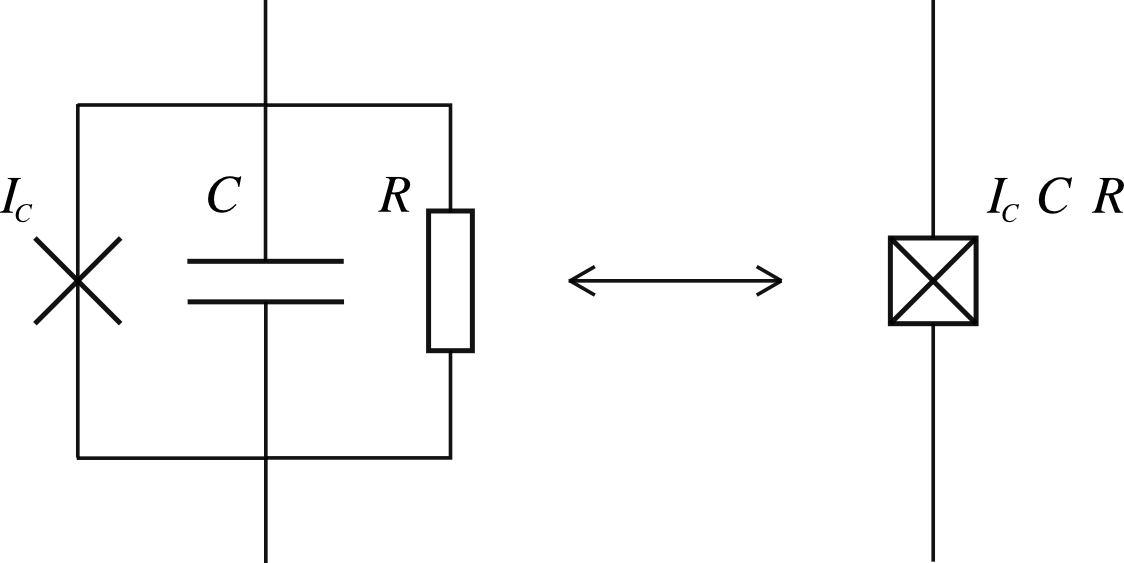
\includegraphics[width=0.65\textwidth]{Pictures/RCSJ.png}
\caption{Схема RCSJ в виде параллельного соединения идеального джозефсоновского перехода с конденсатором и резистором.}
\label{fig:RSCJ}
\end{figure}

Принципиальная схема изображена на \autoref{fig:RSCJ}. В случае, когда ток через систему не превышает критического $I_c$, резистор на схеме может быть опущен. В силу параллельности соединения выполнено также соотношение $\displaystyle \frac{\hbar}{2e}\frac{\partial\varphi}{\partial t} = U_C$ между напряжениями на переходе и на конденсаторе, которое устанавливает аналогию между неидеальным переходом и колебательным контуром с нелинейной индуктивностью.

В рамках RCSJ-модели энергия перехода состоит из энергии, запасенной в нелинейной индуктивности идеального перехода, и энергии конденсатора:
\begin{gather}
E = E_{ind}+E_{cap}  \label{eq:JJenrj1}\\
E_{ind} = \int I_JV_J\, dt = I_c \frac{\hbar}{2e}\int_0^T \sin(\phi(t))\frac{d\phi(t)}{dt}dt \notag\\
= E_J \int_0^\varphi \sin\phi\, d\phi = E_J [1-\cos\varphi] \\
E_{cap} = \frac{1}{2}C U_C^2 = \frac{1}{2} C \left(\frac{\Phi_0}{2\pi}\right)^2 \dot \varphi^2 = 
\frac{\hbar^2}{4E_C} \dot \varphi^2,\ E_C = \frac{(2e)^2}{2C}.
\label{eq:JJenrj2}
\end{gather}
\subsection{Фазо-потоковое соотношение}
Рассмотрим замкнутый сверхпроводящее кольцо конечной толщины, быть может, прерванный конечным числом джозефсоновских переходов $\{J_1..J_n\}$. Рассмотрим применительно к данному случаю уравнение (\ref{eq:lond2}). Проведем контур $C$ внутри кольца так, чтобы он нигде не приближался к стенкам на расстояние, меньшее глубины проникновения магнитного поля (\autoref{fig:ring}). Тогда сверхток на всей его длине будет равен нулю, и, проинтегрировав по нему (\ref{eq:lond2}), мы получим следующее равенство:
\begin{equation}
\oint\displaylimits_C \mathbf{A}d\mathbf{l} = \frac{\Phi_0}{2\pi}\oint\displaylimits_C \nabla \theta d \mathbf{l} \notag.
\end{equation}
Руководствуясь \autoref{fig:ring}, соображениями однозначности волновой функции (\ref{eq:glwf}) при обходе вокруг контура и теоремой Стокса для $\operatorname{rot} \mathbf{A}$, можем написать:
\begin{gather}
\Phi = \frac{\Phi_0}{2\pi}\left(\sum_i \varphi_n + 2\pi k\right) \notag \\
\sum_i \varphi_n = 2\pi\left(\frac{\Phi}{\Phi_0} - k\right),\ k\in \mathcal{Z}.
\label{eq:phsflx}
\end{gather}

\begin{figure}[h]
\centering
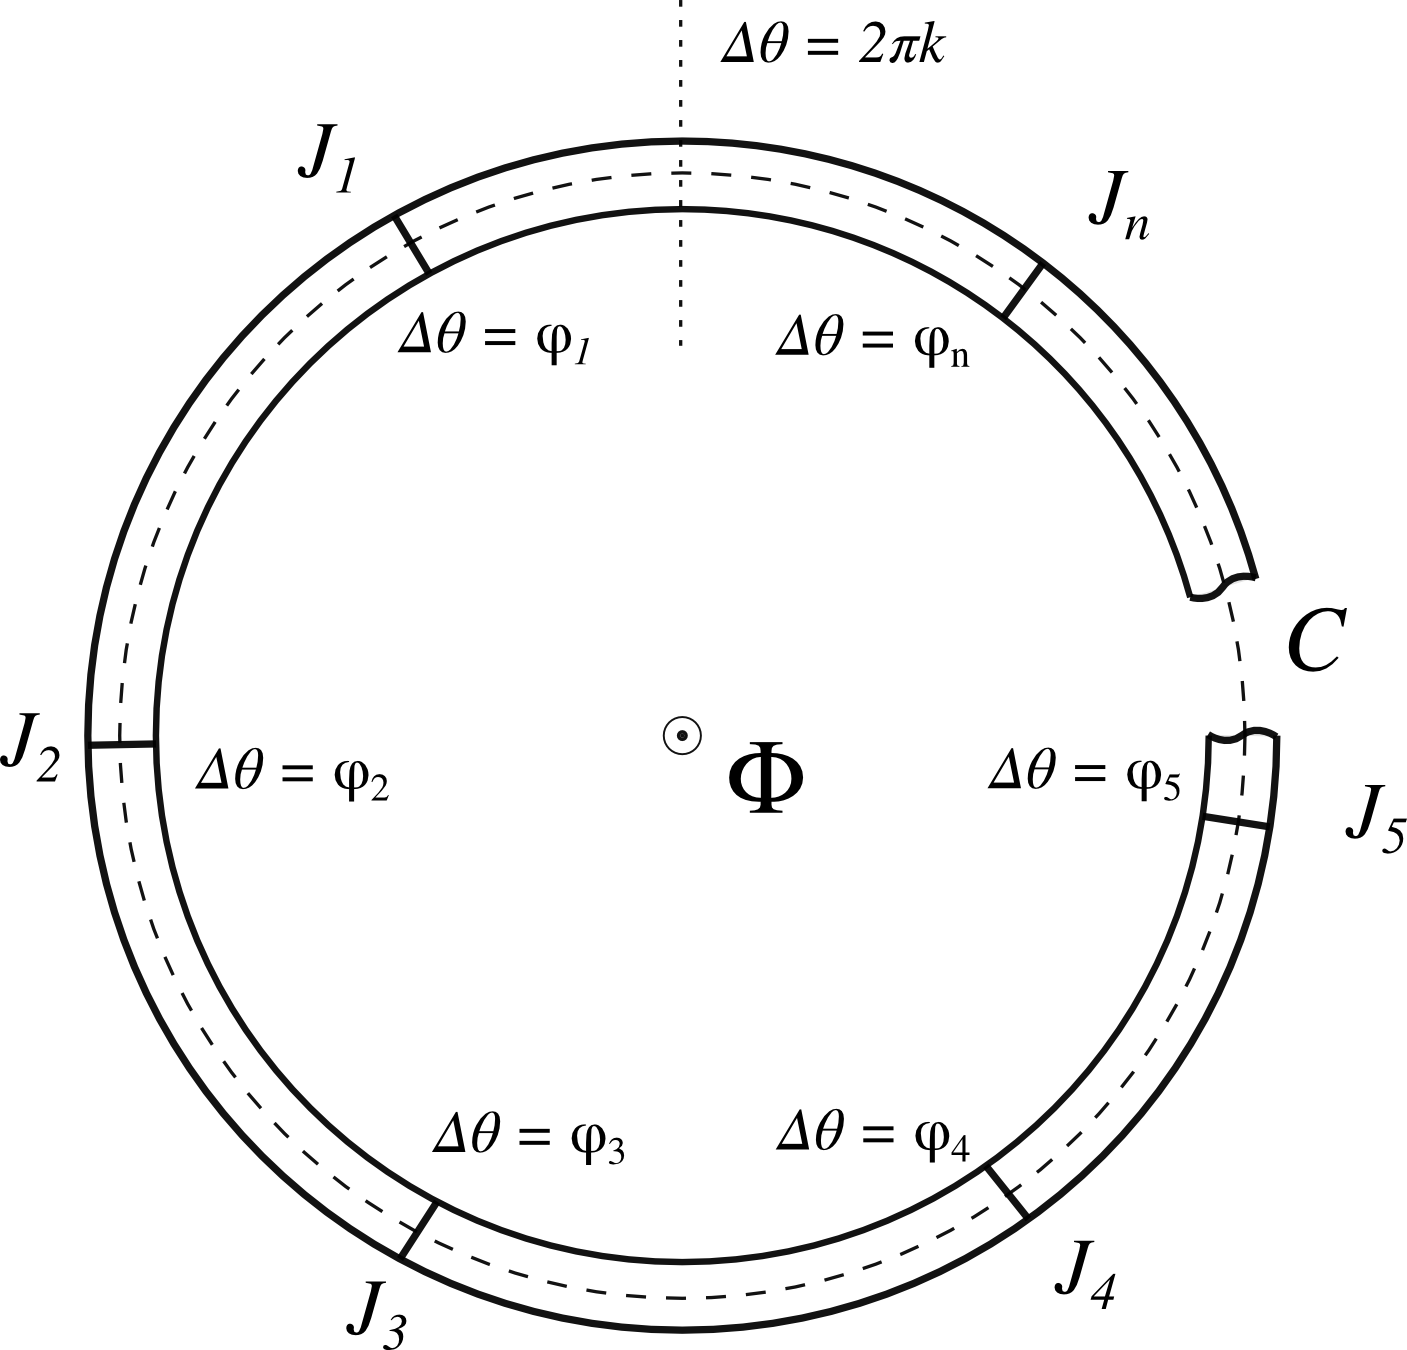
\includegraphics[width=0.5\linewidth]{Pictures/ring.png}
\caption{К выводу фазо-потокового соотношения. Пунктиром обозначен контур интегрирования C. Через $\varphi_i$ обозначены скачки фаз на джозефсоновских контактах, а точками - место разрешенного накопления фазы при полном обходе вокруг кольца $2\pi k,\ k\in\mathcal{Z}$.}
\label{fig:ring}
\end{figure}

Таким образом, получено фазо-потоковое соотношение. Видно, что в случае отсутствия в кольце джозефсоновских переходов полученное уравнение (\ref{eq:phsflx}) опишет равенство магнитного потока $\Phi$, проходящего через сверхпроводящее кольцо, целому числу  k квантов потока $\Phi_0$, обосновывая определение этой константы в (\ref{eq:lond2}).


\section{Теория изолированного Flux-кубита}
Flux-кубит, или потоковый трехконтактный сверхпроводящий кубит, был предложен впервые в 1999 году\cite{Orlando1999} и представляет собой сверхпроводящий контур, прерванный в трех местах джозефсоновскими переходами (\autoref{fig:qubit}), два из которых одинаковы, а третий отличается по площади в $\alpha$ раз. Под \textit{изолированным} в данном разделе понимается одиночный кубит, не взаимодействующий с окружением ни диссипативным, ни консервативным образом. Единственным внешним фактором является при таком рассмотрении постоянное магнитное поле, проходящее через контур.

\begin{figure}
\centering
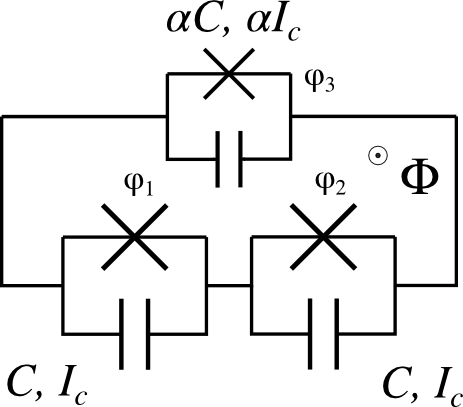
\includegraphics[width=0.4\textwidth]{Pictures/qubit}
\caption{Принципиальная схема Flux-кубита в рамках RCSJ-модели. Два из трех переходов по площади одинаковы, площадь третьего по сравнению с ними в $\alpha$ раз отличается (параметры отличаются в то же число раз согласно формулам для емкости конденсатора и (\ref{eq:Ic})). $\Phi$ -- поток, пронизывающий контур. Резисторы не изображены, так как рабочий ток переходов меньше $I_c$.}
\label{fig:qubit}
\end{figure}

\subsection{Построение гамильтониана}
Для того, чтобы провести квантово-механическое рассмотрение кубита, требуется записать его гамильтониан. Для этого прежде всего нужно понять, какими независимыми степенями свободы он обладает. Вообще говоря, состояние одиночного джозефсоновского перехода, в силу того, что в параллельном соединении RCSJ-модели $U = \frac{\hbar}{2e}\dot\varphi$, целиком описывается своей разностью фаз. Для трех невзаимодействующих переходов таких разностей будет три, и их и следует выбрать в качестве обобщенных координат системы. Однако в случае замкнутого контура дополнительно накладывается фазо-потоковое соотношение (\ref{eq:phsflx}):
\begin{equation}
\varphi_1 + \varphi_2 + \varphi_3 = 2\pi\left(\frac{\Phi}{\Phi_0} - k\right),\ k\in \mathcal{Z}.
\label{eq:qubit_phsflx}
\end{equation}
Таким образом, в контуре на \autoref{fig:qubit} остаются независимыми только две разности фаз из трех. Введя их в качестве обобщенных координат, можно понять, что является аналогом кинетической, а что -- потенциальной энергии системы. В уравнениях (\ref{eq:JJenrj1})-(\ref{eq:JJenrj2}) энергия перехода зависит непосредственно от $\varphi$, а емкостная от $\dot \varphi$. Таким образом, переход запасает потенциальную, а емкость кинетическую энергию. Энергия магнитного поля, возникающего при течении тока в кольце, считается малой в силу малости геометрической индуктивности кубита по сравнению с джозефсоновской индуктивностью переходов, а поток $\Phi = \Phi_{ext}$ (подробное описание данной процедуры см. в статье \cite{Robertson2006}). Теперь можно записать лагранжиан системы, используя все те же уравнения (\ref{eq:JJenrj1})-(\ref{eq:JJenrj2}) и выражая разность фаз $\varphi_3$ отличающегося перехода через разности фаз $\varphi_1$ и $\varphi_2$ одинаковых переходов при помощи (\ref{eq:qubit_phsflx}):
\begin{gather*}
\mathcal{L} = \mathcal{T}-\mathcal{U}, \\
\mathcal{T} = E_{cap} =\frac{1}{2}\sum_{i=1}^3 C_i V_i^2 = \frac{1}{2} \left(\frac{\Phi_0}{2\pi}\right)^2 \left[C(\dot \varphi_1)^2 + \alpha C \left(\dot \varphi_1 + \dot\varphi_2\right)^2 + C(\dot \varphi_2)^2\right] \\
= \frac{1}{2}\left(\frac{\Phi_0}{2\pi}\right)^2 \left(\begin{matrix}
\dot\varphi_1 &\dot\varphi_2
\end{matrix}\right) C \left(\begin{matrix}
1+\alpha & \alpha \\
\alpha & 1+\alpha
\end{matrix}
\right)
\left(\begin{matrix}
\dot\varphi_1 \\
\dot\varphi_2
\end{matrix}\right),\\
\mathcal{U} = E_{ind} = E_J\left[2+\alpha + \cos\varphi_1 + \cos\varphi_2 + \alpha \cos\left(2\pi\frac{\Phi}{\Phi_0} - \varphi_1 - \varphi_2 \right)\right].
\end{gather*}
Строить гамильтониан системы из такого лагранжиана не очень удобно, поэтому предварительно произведем замену координат $\displaystyle \phi = \frac{\varphi_1 + \varphi_2}{2},\ \theta = \frac{\varphi_1 - \varphi_2}{2}$:
\begin{gather}
\mathcal{T}  \overset {\varphi_1, \varphi_2 \rightarrow \phi, \theta}{=}
C\left(\frac{\Phi_0}{2\pi}\right)^2 (\begin{matrix}
\dot \phi & \dot \theta
\end{matrix})
\left(\begin{matrix}
1+2\alpha & 0\\
0 & 1
\end{matrix}
\right)
\left(\begin{matrix}
\dot \phi \\ \dot \theta
\end{matrix}\right), \notag
\\
\mathcal{U} \overset {\varphi_1, \varphi_2 \rightarrow \phi, \theta}{=} E_J\left[2+\alpha - 2\cos(\phi)\cos(\theta) - \alpha\cos\left(2\pi\frac{\Phi}{\Phi_0} -2\phi\right)\right].
\label{eq:U_qb}
\end{gather}
Теперь, стандартным образом вводя обобщенный импульс 
$\displaystyle \mathbf{p}^T = \left(\begin{matrix}p_\phi & p_\theta\end{matrix}\right) = \left(\begin{matrix}\frac{\partial\mathcal{L}}{\partial\dot\phi} & \frac{\partial\mathcal{L}}{\partial\dot\theta}\end{matrix}\right)$ и производя преобразование Лежандра, получим итоговый гамильтониан системы:
\begin{gather*}
\mathcal{H} = \frac{p_\phi^2}{2M_\phi} + \frac{p_\theta^2}{2M_\theta}+ E_J\left[2+\alpha - 2\cos(\phi)\cos(\theta) - \alpha\cos\left(2\pi\frac{\Phi}{\Phi_0} -2\phi\right)\right], \\
M_\phi = 2C\left(\frac{\Phi_0}{2\pi}\right)^2(1+2\alpha),\ M_\theta = 2C\left(\frac{\Phi_0}{2\pi}\right)^2.
\end{gather*}
Далее, осуществляя переход к операторному виду квантовой механики, можно получить оператор Гамильтона для сверхпроводящего потокового кубита в терминах исключительно $E_C$ и $E_J$:
\begin{gather}
\hat{\mathcal{H}} = E_C\left[-\frac{1}{2(1 + 2\alpha)}\frac{\partial^2}{\partial\phi^2} 
- \frac{1}{2}\frac{\partial^2}{\partial\theta^2}\right]+ E_J\left[2+\alpha - 2\cos(\phi)\cos(\theta) - \alpha\cos\left(2\pi\frac{\Phi}{\Phi_0} -2\phi \right)\right].
\label{eq:hamiltonian}
\end{gather}

\subsection{Квантово-механический анализ}

\begin{figure}[!p]
\begingroup
\captionsetup[subfigure]{width=0.95\textwidth}
\centering
\begin{subfigure}[t]{0.49\linewidth}
\centering
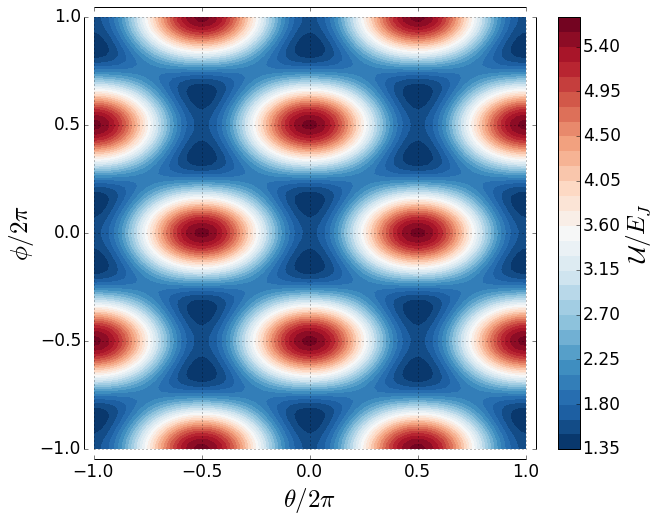
\includegraphics[height = .8\textwidth]{Pictures/qubit_potential}
\caption{Трехмерное изображение потенциала при $\Phi = \Phi_0/2,\ \alpha=0.8$. Можно видеть $2\pi$-периодическую решетку из двойных ям.}
\label{fig:U3d}
\end{subfigure}~
\begin{subfigure}[t]{0.49\linewidth}
\centering
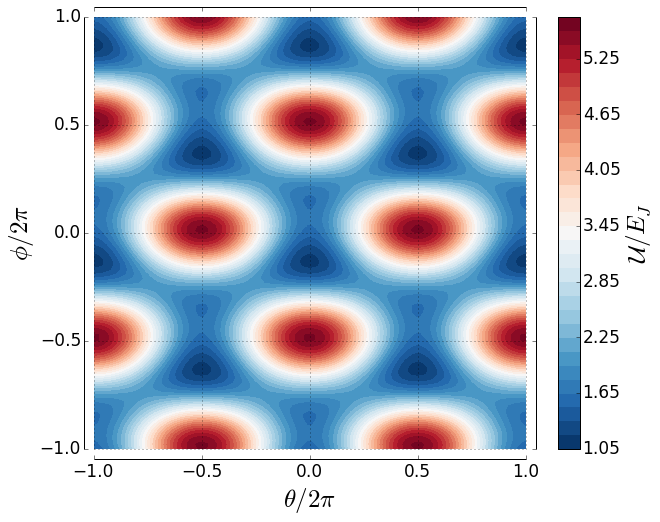
\includegraphics[height = .8\textwidth]{Pictures/qubit_potential2}
\caption{При отклонении потока от $\Phi_0/2$ появляется перекос внутри двойных ям, одна половина становится глубже, а другая мельче в зависимости от знака отклонения $\Delta\Phi$. Здесь $\Delta\Phi=-0.05\Phi_0$.}
\label{fig:U3d2}
\end{subfigure}
\begin{subfigure}[t]{0.49\linewidth}
\centering
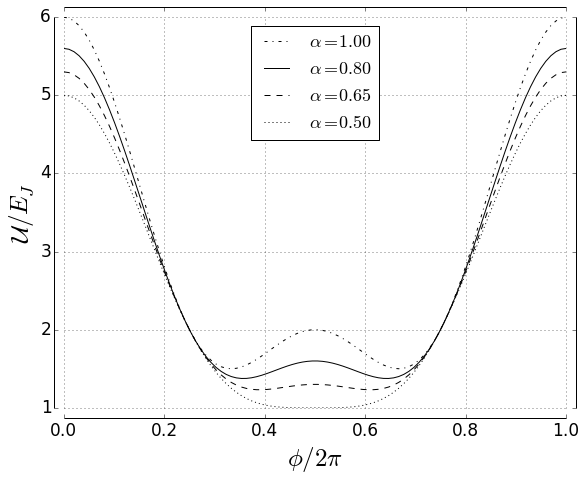
\includegraphics[height = 0.8\textwidth]{Pictures/qubit_potential_cut}
\caption{Срез потенциала при $\Phi = \Phi_0/2$ по направлению $\theta = \pi$ (барьер внутри ям) в зависимости от $\alpha$. При $\alpha = 0.5$ этот барьер пропадает, при $\alpha=1$ он сравнивается с барьером между ямами (см. (\subref{fig:U_cut2})).}
\label{fig:U_cut}\quad
\end{subfigure}
\begin{subfigure}[t]{0.49\linewidth}
\centering
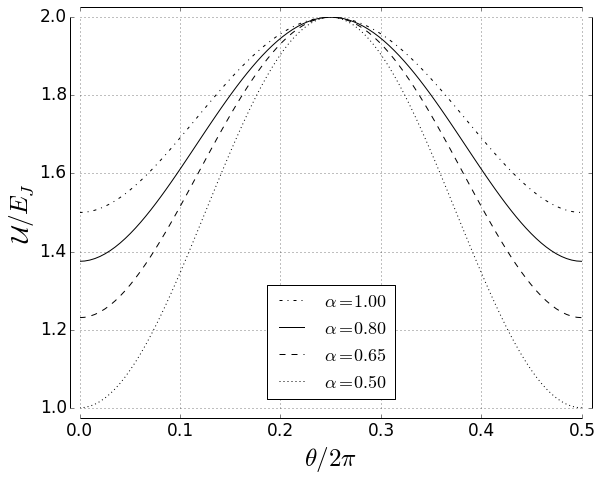
\includegraphics[height = 0.8\textwidth]{Pictures/qubit_potential_cut2}
\caption{Срез потенциала при $\Phi = \Phi_0/2$ по направлению $\phi = \left(1 - \frac{2}{\pi}\arccos
\frac{1}{2\alpha}\right)\theta+\arccos\frac{1}{2\alpha}$ (барьер между ямами) в зависимости от $\alpha$. Здесь крайние точки отвечают минимумам $\mathcal{U}$ при $\theta=0\ (\pi),\ \phi=\arccos
\frac{1}{2\alpha}\ \left(\pi - \arccos\frac{1}{2\alpha}\right)$.}
\label{fig:U_cut2}
\end{subfigure}
\endgroup
\caption{Графическое изображение периодического потенциала Flux-кубита в зависимости от относительного размера отличающегося перехода $\alpha$ и пронизывающего потока $\Phi$.}
\label{fig:U_fq}
\end{figure} 

\paragraph{Анализ потенциала.} Прежде всего рассмотрим потенциал $\mathcal{U}(\phi, \theta)$. На \autoref{fig:U_fq} представлены графики, демонстрирующие его структуру в случае $\Phi = \Phi_0/2$, или в так называемой \textit{точке вырождения} по потоку. На \autoref{fig:U_fq}~(\subref{fig:U3d}) можно видеть, что потенциал $2\pi$-периодичен по каждой из переменных $\phi$ и $\theta$ и представляет собой бесконечную решетку из симметричных двойных ям, отделенных друг от друга диагональными барьерами. Каждая их ям, в свою очередь, делится на две части меньшим барьером. Его высота, как видно из \autoref{fig:U_fq}~(\subref{fig:U_cut}), определяется параметром $\alpha$. Для того, чтобы структура оставалась подобной изображенной на \autoref{fig:U_fq}~(\subref{fig:U3d}), требуется, чтобы $\alpha\in(0.5,\ 1)$: при нарушении этого условия либо совсем пропадает внутренний барьер, либо внешний барьер сравнивается с внутренним по высоте, и ямы перестают быть качественно отделены друг от друга (\autoref{fig:U_fq}~(\subref{fig:U_cut2})). Минимумы $\mathcal{U}$ находятся в точках $\theta=\pi k,\ \phi=\pm\arccos\frac{1}{2\alpha}+\pi n,\ k,\ n\in\mathcal{Z}$, причем в точке вырождения все минимумы имеют одинаковую энергию, а при отходе от нее в зависимости от знака отклонения одна половина двойных ям становится мельче, а другая глубже, и вырождение внутри каждой ямы снимается (\autoref{fig:U_fq}~(\subref{fig:U3d2})). 

\begin{figure}[!p]
\begingroup
\captionsetup[subfigure]{width=\textwidth}
\centering
\begin{subfigure}[t]{0.75\linewidth}
\centering
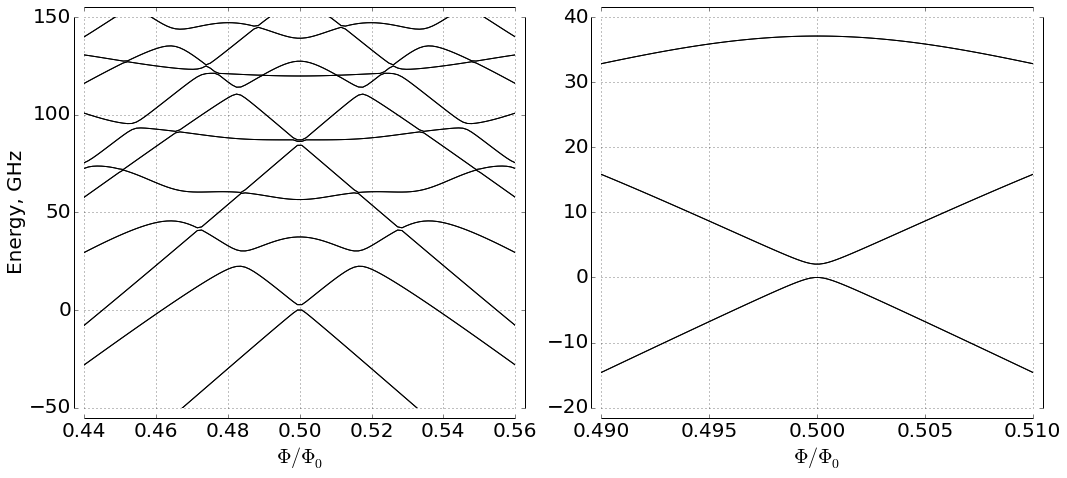
\includegraphics[width = \textwidth]{Pictures/qubit_levels}
\caption{Уровни энергии в зависимости от внешнего поля. Каждая линия на рисунке на самом деле является двойной (объяснение см. в тексте).}
\label{fig:levels}
\end{subfigure}

\begin{subfigure}[t]{0.8\linewidth}
\centering
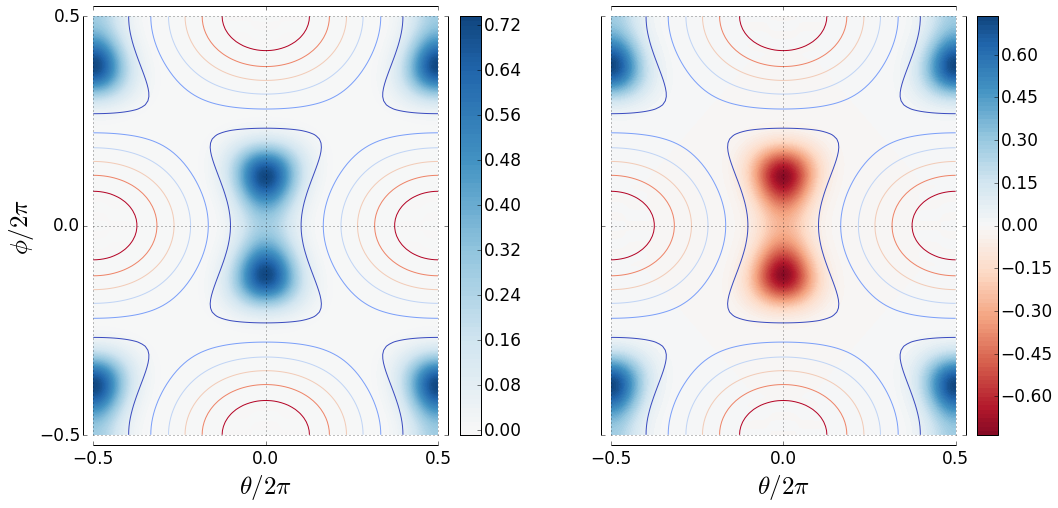
\includegraphics[width = \textwidth]{Pictures/wfs01}
\caption{Граничные состояния нулевой зоны (``$\ket{g}$-состояния'') в точке вырождения. Внутри ям волновая функция четная.}
\label{fig:wfs01}
\end{subfigure}

\begin{subfigure}[t]{0.8\linewidth}
\centering
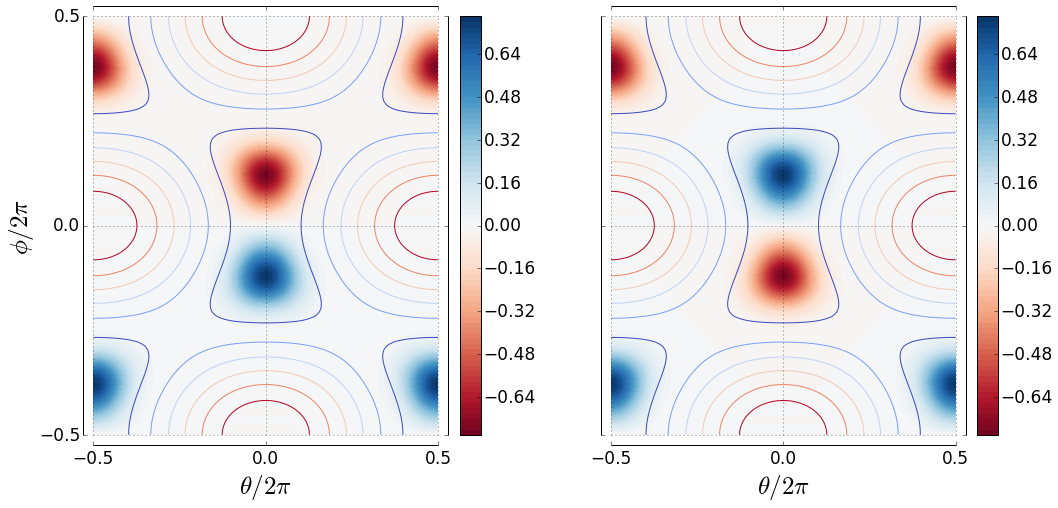
\includegraphics[width = \textwidth]{Pictures/wfs23}
\caption{Граничные состояния первой зоны (``$\ket{e}$-состояния'') в точке вырождения. Внутри ям волновая функция нечетная.}
\label{fig:wfs23}
\end{subfigure}

\endgroup
\caption{Результаты численного решения стационарного уравнения Шредингера с параметрами $\alpha=0.7,\ E_J  = 30E_C = 400\ \text{GHz}$. Цветом обозначено значение волновой функции, нормированной на единицу в периоде потенциала.}
\label{fig:numerical_res}
\end{figure} 

\paragraph{Стационарные состояния.} Прежде, чем начинать поиск стационарных состояний для гамильтониана (\ref{eq:hamiltonian}), важно не упустить одну особенность. Строго говоря, в силу того, что потенциал (\ref{eq:U_qb}) является периодическим, решениями уравнения Шредингера будут являться \textit{блоховские функции}, а спектр энергий будет иметь зонную структуру. Таким образом, как это ни удивительно, один Flux-кубит представляет собой модель частицы в идеальной периодической решетке двумерного твердого тела. Для приближенного аналитического решения задачи в случае, когда $E_J \gg E_C$, можно использовать модель сильной связи для центрированной решетки с базисом, однако здесь мы будем рассматривать численный вариант. 

Для нахождения стационарных состояний гамильтониана (\ref{eq:hamiltonian}) может быть применен метод, изложенный в работе\cite{Johansson}. Используя периодичность, можно разложить в ряд Фурье и потенциал, и искомую волновую функцию, ограничиваясь $2N+1$ начальными слагаемыми в разложении, и подставить их в уравнение Шредингера с гамильтонианом (\ref{eq:hamiltonian}), что после определенных преобразований сведет задачу к поиску собственных значений и векторов матрицы $(2N+1)^2$ на $(2N+1)^2$. Результаты такого вычисления для $N=20$ представлены на \autoref{fig:numerical_res}. Вычисленный спектр энергий состоит из дублетов (на рисунке они сливаются в синглеты), причем расщепление в дублетах обусловлено разными периодическими конфигурациями волновой функции при фиксированной четности ее внутри ям, а расстояния между дублетами изменением четности внутри ям. Это происходит так как используемый машинный метод ``вылавливает'' границы энергетических зон, так как может найти только чисто действительные блоховские решения. Действительно, по теореме Блоха $\psi(r) = e^{ikR}\psi(r)$, для граничных квазиимпульсов $k = 0$  и $k = K/2$ выполнено соответственно $\psi(r+R) = \psi(r)$ и $\psi(r+R)=-\psi(r)$, что и наблюдается на парах \autoref{fig:numerical_res}~(\subref{fig:wfs01}) и \autoref{fig:numerical_res}~(\subref{fig:wfs23}). 
Видно также, что четные конфигурации волновой функции имеют меньшую энергию, а нечетные большую, в соответствии с вышесказанным.

В зависимости от поля спектр ведет себя, как показано на \autoref{fig:numerical_res}~(\subref{fig:levels}), неравномерно: в окрестности $\Phi_0/2$ четные пары уровней сдвигаются вниз, нечетные вверх, а на большем удалении магнитного потока от полкванта картина вообще теряет порядок из-за значительного числа квазипересечений. На \autoref{fig:numerical_res}~(\subref{fig:wfs01}) и (\subref{fig:wfs23}) изображены соответственно нулевое и первое дублетные состояния в точке вырождения.  Далее мы будем пренебрегать тем, что первые две зоны отличны от дискретных уровней, так как расщепления внутри них примерно в $10^5$ раз меньше, чем расстояния между ними, и назовем верхнюю по энергии зону ``$\ket{e}$-состоянием'', а нижнюю ``$\ket{g}$-состоянием''.

\paragraph{Двухуровневое приближение.} Следующим шагом будет приведение системы к двум нижним состояниям, пренебрегая всеми остальными. Это оправданно, так как третий дублет в точке вырождения лежит гораздо выше (почти в 20 раз) по энергии, чем состояние $\ket{e}$ . Так же одновременно с этим мы явно выделим в гамильтониане член, отвечающий воздействию отклонения потока от полкванта, разложив в ряд Тейлора последнее слагаемое в потенциале. Это также оправданно потому, что, как видно из \autoref{fig:numerical_res}~(\subref{fig:levels}), для большого изменения расстояния между уровнями годится даже малое отколнение от $\Phi_0/2$. Итак, записываем разложение потенциала и полный гамильтониан в матричной форме (в базисе из состояний $\ket{g}$ и $\ket{e}$ в точке вырождения):
\begin{gather}
\hat{\mathcal{U}} = E_J\left[2+\alpha - 2\cos(\phi)\cos(\theta) - \alpha\cos\left(2\pi\frac{\Phi_0/2+\delta\Phi}{\Phi_0} -2\phi \right)\right] = \notag \\
= E_J\left[2+\alpha - 2\cos(\phi)\cos(\theta) - \alpha\cos\left(\pi - 2\phi \right)\right] + \alpha E_J\sin\left(\pi - 2\phi\right)\ 2\pi\frac{\delta\Phi}{\Phi_0} + \mathcal{O}(\delta\Phi^2), \notag \\
\left(\begin{matrix}
\mathcal{H}_{11} & \mathcal{H}_{12} \\
\mathcal{H}_{21} & \mathcal{H}_{22}
\end{matrix}\right) = 
\hat{\mathcal{T}} + \hat{\mathcal{U}} + \alpha E_J 	
\left(\begin{matrix}
\bra{0}\sin(\pi - 2\phi)|\ket{0} & \bra{0}\sin(\pi - 2\phi)\ket{1}\\
\bra{1}\sin(\pi - 2\phi)\ket{0} &\bra{1}\sin(\pi - 2\phi)\ket{1}
\end{matrix}\right)2\pi\frac{\delta\Phi}{\Phi_0} = \notag \\  \vspace{50pt}
= \frac{\varepsilon}{2}\,\hat\sigma_z + \frac{\delta}{2}\,\hat\sigma_x ,\ket{g}_{\Phi_0/2}=\rbrkt{\begin{matrix}
1\\0\end{matrix}},\ \ket{e}_{\Phi_0/2}=\rbrkt{\begin{matrix}
0\\1\end{matrix}},
\label{eq:trunc_hamilonian}
\end{gather}
где $\varepsilon$ -- расстояние между уровнями, а $\delta = 4\pi\alpha E_J \delta\Phi/\Phi_0 \cdot C$, $C=const$ -- неизвестный
 коэффициент. Последнее равенство перед (\ref{eq:trunc_hamilonian}) верно, так как при $\Phi = \Phi_0/2$ диагональные матричные элементы равны нулю в силу нечетности оператора $\sin(\pi - 2\phi)$ и симметрии волновых функций на \autoref{fig:numerical_res}, а элементы на побочной диагонали равны в силу самосопряженности этого оператора и действительности волновых функций как собственных для гамильтониана. Самосопряженность легко выводится из физического смысла данного оператора -- это оператор тока через меньший переход $\hat{I}_3$. Равенство нулю его среднего значения в состояниях $\ket{g}$ и $\ket{e}$ при $\Phi = \Phi_0/2$ означает, что в точке вырождения в кубите не течет незатухающий ток. Этим объясняется ослабление в таком режиме его взаимодействия со средой -- кубит не создает полей.

Сокращенный гамильтониан \eqref{eq:trunc_hamilonian} можно просто привести к диагональному виду. Его собственные значения и их разность будут зависеть от $\delta$, и, следовательно, от $\Phi$ следующим образом:
\begin{equation}
E_{1, 2} = \pm \frac{1}{2}\sqrt{\varepsilon^2 + \delta^2},\
\Delta E = h \nu_q = \sqrt{\varepsilon^2 + \delta^2},
\end{equation}
где $\nu_q$ -- это экспериментально наблюдаемая частота перехода между кубитными уровнями. Легко построить зависимость этой частоты от приложенного поля -- это гипербола, причем по ее асимптотам можно вычислить константу связи с внешним постоянным полем.

\newpage
\part{Экспериментальная часть}
\part{Результаты}
\part{Заключение}

\bibliographystyle{ugost2008}
\bibliography{Thesis.bib}

\end{document}